\documentclass[12pt, a4paper, oneside]{ctexart}
\usepackage{amsmath, amsthm, amssymb, bm, color, framed, graphicx, hyperref, mathrsfs}
\usepackage{amsfonts}
\usepackage{fancyhdr}
\usepackage{graphicx}
\pagestyle{fancy}
\lfoot{}%这条语句可以让页码出现在下方


\title{\textbf{第七次课程作业}}
\author{张浩然 023082910001}
\date{\today}
\linespread{1.5}
\definecolor{shadecolor}{RGB}{241, 241, 255}
\newcounter{problemname}
\newenvironment{problem}{\begin{shaded}\stepcounter{problemname}\par\noindent\textbf{题目\arabic{problemname}. }}{\end{shaded}\par}
\newenvironment{solution}{\par\noindent\textbf{解答. }}{\par}
\newenvironment{note}{\par\noindent\textbf{题目\arabic{problemname}的注记. }}{\par}

\begin{document}

\maketitle

\begin{problem}
    43. 证明$Householder$变换$H_v$是关于超平面$v^\perp $的反射,从而是正交变换.试画出三维$Householder$变换的示意图.
\end{problem}


\begin{solution}
    设$u \in v^\perp$,则$u \cdot v=0$,$H_v(u)=u$

    设$w$是超平面外的任意向量,则$w=u+\lambda v$,其中$\lambda \in \mathbb{R}$,则$H_v(w)=-w$

    因此$Householder$变换是镜面反射正交变换.

    \begin{figure}[h]
        \centering
        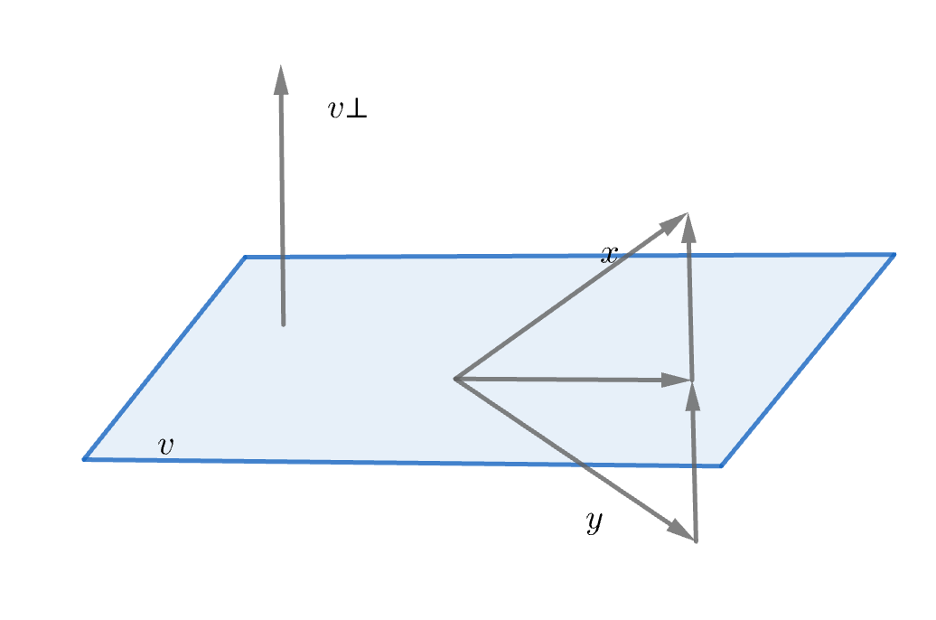
\includegraphics[width=0.5\textwidth]{Picture1.png}
        \caption{三维图示}
    \end{figure}
        
\end{solution}

%%%%%%%%%%%%%%%%%%%%%%%%%%%%%%%%%%%%%%
\begin{problem}
    2.设  $A$  为第一章\textbf{例1.2.2} 中的矩阵,
    
    (1) 利用满秩分解和$ Sylvester $降幂公式求 $ A $ 的特征多项式与 $ A^{6} $;
    
    (2) 求与 $ A$  相似的分块对角矩阵, 使得每块恰有唯一的特征值.
\end{problem}

\begin{note}
    
    \textbf{例 1.2.2}
    $A=\left(\begin{array}{ccccc}3 & -1 & 3 & 2 & 5 \\5 & -3 & 2 & 3 & 4 \\1 & -3 & -5 & 0 & -7 \\2 & -2 & -1 & 1 & -1\end{array}\right)$
    
    \textbf{例 1.2.3}
    $A=\left(\begin{array}{llll}-3 & 2 & -2 & 3 \\-2 & 1 & -1 & 2 \\-2 & 2 & -2 & 2 \\-1 & 1 & -1 & 1\end{array}\right)$
\end{note}

\begin{solution}
    ps.\textbf{例 1.2.2}无法使用降幂公式,应该为\textbf{例1.2.3}

    (1). 由于
        
        $A=\left(\begin{array}{ll}-3 & 2 \\-2 & 1 \\-2 & 2 \\-1 & 1\end{array}\right)\left(\begin{array}{cccc}1 & 0 & 0 & -1 \\0 & 1 & -1 & 0\end{array}\right)=L R$
        
        故  
        
        $|\lambda I-A|=|\lambda I-L R|=\lambda^{2}|\lambda I-R L|=\lambda^{2}(\lambda+1)(\lambda+2) .$ 
        
        $A^n=(LR)^n=L(RL)^{n-1}R$

        所以$A^{6}=\left(\begin{array}{cccc}96 & -95 & 95 & -96 \\ 64 & 63 & -63 & -64 \\ 64 & -64 & 64 & -64 \\ 32 & -32 & 32 & -32\end{array}\right) $.
    
    (2).计算$Jordan$标准型得
    $J=\left(\begin{array}{cccc}0 & 0 & 0 & 0 \\0 & 0 & 0 & 0 \\0 & 0 & -2 & 0 \\0 & 0 & 0 & -1\end{array}\right)$.
    \end{solution}
%%%%%%%%%%%%%%%%%%%%%%%%%%%%%%%%%%%%%%%
\begin{problem}
    3.设 $\alpha=\left(a_{1}, \cdots, a_{n}\right)^{\mathrm{T}}, \beta=\left(b_{1}, \cdots, b_{n}\right)^{\mathrm{T}}$, $x$为任意常数, $ A=xI_{n}+\alpha \beta^{\mathrm{T}}$ .
    
    (1) 直接计算行列式 $ |A| $;
    
    (2) 利用 $Sylvester$ 降幂公式计算行列式 $ |A| $;
    
    (3) 利用特征值计算行列式 $ |A| $.
\end{problem}
\begin{solution}
    (1).
    $
    A=|xI_n+\alpha\beta^T|=
    \left | \begin{matrix}
        a_1b_1+x &a_1b_2  &a_1b_3 &\cdots &a_1b_n \\
        a_2b_1 &a_2b_2+x &a_2b_3 &\cdots &a_2b_n \\
        \vdots & \vdots &\ddots &\ddots &\vdots  \\
        a_nb_1 &a_nb_2 &a_nb_3 &\cdots &a_nb_n+x \\
    \end{matrix} \right | 
    =
    \left | \begin{matrix}
        1 & b_1 &b_2 &b_3&\cdots &b_n \\
        0&a_1b_1+x &a_1b_2  &a_1b_3 &\cdots &a_1b_n \\
        0&a_2b_1 &a_2b_2+x &a_2b_3 &\cdots &a_2b_n \\
        \vdots& \vdots & \vdots &\ddots &\ddots &\vdots  \\
        0&a_nb_1 &a_nb_2 &a_nb_3 &\cdots &a_nb_n+x \\
    \end{matrix} \right |
    = 
    \left | \begin{matrix}
        1 & b_1 &b_2 &b_3&\cdots &b_n \\
        -a_1&x &0  &0 &\cdots &0 \\
        -a_2&0 &x &0 &\cdots &0 \\
        \vdots& \vdots & \vdots &\ddots &\ddots &\vdots  \\
        -a_n&0&0 &0 &\cdots &x \\
    \end{matrix} \right |
    =x^n(1+\frac{\beta^T\alpha}{x})
    $

    (2).$|A|=\left|x I_{n}+\alpha \beta^{T}\right|=x^{n-1}\left|x+\beta^{T} \alpha\right|=x^{n-1}\left(x+\beta^{T} \alpha\right)$

    (3).矩阵 $A$的特征值有$n-1$个$x$一个$x+\beta^T\alpha$,所以$|A|=x^{n-1}(x+\beta^T\alpha)$
\end{solution}
%%%%%%%%%%%%%%%%%%%%%%%%%%%%%%%%%%%%%%
\begin{problem}
   5.(1)举例说明$Schur$三角化定理在实数域上不成立.
\end{problem}

\begin{solution}
   $\begin{pmatrix}
         0& -1 \\
         1 & 0
   \end{pmatrix}$
\end{solution}
%%%%%%%%%%%%%%%%%%%%%%%%%%%%%%%%%%%%%%
\begin{problem}
    11.求下列矩阵的最小多项式并指出其中可以对角化的矩阵:
    
    (1)  $\left(\begin{array}{ll}3 & 2 \\ 4 & 5\end{array}\right)$ ;
    (2)  $\left(\begin{array}{ccc}2 & 3 & 2 \\ 0 & 5 & 4 \\ 0 & -2 & -1\end{array}\right) $;
    (3)  $\left(\begin{array}{ccc}4 & 6 & 0 \\ -3 & -5 & 0 \\ 3 & 6 & 1\end{array}\right) $;
    (4)  $\left(\begin{array}{ccc}4 & 6 & 0 \\ -3 & -5 & 0 \\ -3 & 6 & 1\end{array}\right) $.
\end{problem}

\begin{solution}
    (1) $|\lambda I-A|=(\lambda-3)(\lambda-5)-8=(\lambda-1)(\lambda-7)$,所以最小多项式为$(\lambda-1)(\lambda-7)$无重根,可对角化.

    (2) 最小特征多项式$(\lambda-2)(\lambda-3)(\lambda-1)$无重根,可对角化.

    (3)最小特征多项式$(\lambda+2)(\lambda-1)$无重根,可对角化.

    (4)最小特征多项式$(\lambda+2)(\lambda-1)^2$有重根,不可对角化.
\end{solution}
% \begin{note}
%     这里是注记. 
% \end{note}

\end{document}